\documentclass[a4paper]{article}%twocolumn,
\usepackage{graphicx,color}
\usepackage{natbib}
\bibliographystyle{plainnat}
\title{Applying reinforcement learning to Tetris}
\author{Donald Carr\thanks{Sponsored by Microsoft, Telkom, Thrip, Comverse, Verso and Business Connexion} \\ Department of Computer Science \\ Rhodes University \\ Grahamstown 6139,South Africa \\ g02c0108@campus.ru.ac.za}
\date{\today}
\begin{document}
\maketitle
\begin{abstract}
This paper investigates the possible application of reinforcement learning to Tetris. The author investigates the background of Tetris, and qualifies it in a mathematical context. The author discusses reinforcement learning, and considers historically successful applications of it. Finally the author discusses considerations surrounding implementation. 
\end{abstract}

\section{Introduction}

Tetris is a very popular game that was created in 1985 by Alexey Pajitnov and has been ported to nearly every operating system and hardware platform in existence. The incredible popularity and non-trivial nature of the game have led to a large amount of research, both into the maths surrounding the game and into the training of AI entities to play it skillfully. The simplicity of specifying Tetris, along with its ubiquitous existence across systems, lends it to AI research.

Reinforcement learning is a well established\footnote{For a broad history see \citep{suttonbarto}} branch of artificial learning that distinguishes itself from other varieties of artificial intelligence in its focus on trial and error learning, and is an incredibly active area of research. It promises an unprejudiced agent capable of developing its own tactics and realising trends that are implicit in its interactions with the environment. 

This literature review investigates the applicability of reinforcement learning to Tetris. A formal definition of Tetris is presented, along with some of its intricacies. Existing artificial intelligence Tetris players are also investigated, along with the successful applications and deeper qualities of reinforcement learning.

\clearpage

\section{Tetris}

\begin{figure}[h]
\centering%
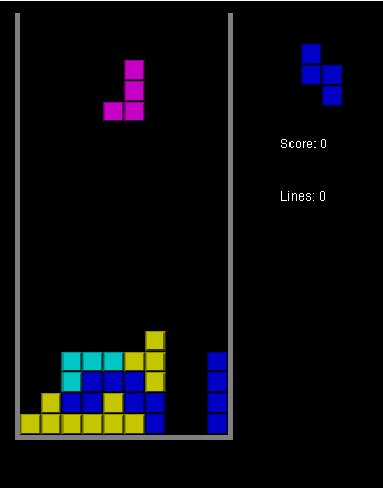
\includegraphics[width=2in]{tetgame.jpg}
\caption{Tetris game in progress}
\label{fig:tetgame}
\end{figure}

Tetris is so well established that it's name has basically lent itself to any entire genre of puzzle games. It has been implemented across such a variety of platforms and over such a span of years, that variations have flourished and "Tetris" refers to a wealth of subtly different games. All variations have a range of different tetrominoes (see Figure \ref{fig:pieces} for examples), which are fixed geometric forms comprised of regular square blocks. These tetrominoes can be rotated and translated in the absence of obstructions. A  single tetromino is selected by the game and appears in the top centre block of a fixed sized discrete well. The tetromino descends at a discrete fixed rate, that is determined by the current difficultly level, until it meets an obstruction. The tetromino is fixed in place if the contact still exists in the descent step following initial contact with an obstruction. If in being fixed it completes a row, the row is completely removed and the entire well contents above the deleted row are shifted downwards one row.

Many different artificial intelligence approaches have been applied to Tetris, and in order to remove implementation discrepancies in gauging the success of the relative algorithms, at least one set of formal guidelines has be specified for generic Tetris. The agent, given the successful application of reinforcement learning, will therefore achieve results which will be directly comparable with those attained by other implementations following the same specifications. The standards set forth by \cite{tetstand} were selected as there is a fair amount of existing Tetris AI research associated with them and they seem reasonable, intuitive and comprehensive.

\subsection{Formal Tetris Specification \citep{tetstand}} 
\begin{itemize}
\item{Tetris has a board with dimensions 10 x 20}
\item{Tetris has seven distinct pieces (See Figure \ref{fig:pieces})}
\item{The current game piece is drawn from a uniform distribution of these seven pieces}
\item{Points are awarded for each block that is landed (not for completing rows)}
\item{The player scores the most points possible for each piece by executing a drop before one or more free-fall iterations transpire}
\item{The game has ten different difficultly settings, which determine the period of free-fall iterations, and are applied as row completion passes certain thresholds}
\end{itemize}

\begin{figure}[h]
\centering
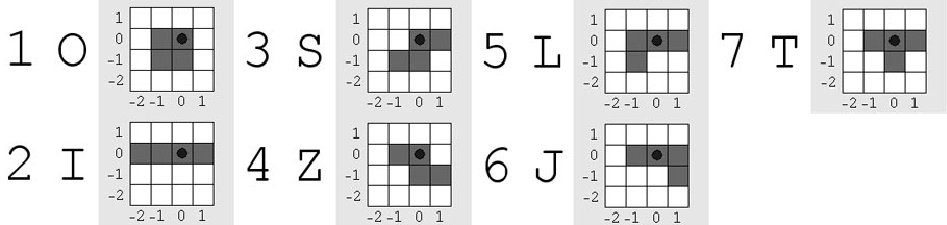
\includegraphics[width=\textwidth]{tetrisblocks.jpg}
\caption{The range of complete Tetris pieces}
\label{fig:pieces}
\end{figure}

\subsection{Further investigation}

It will certainly be interesting to benchmark the agent against existing AI methods, however the limitations imposed by the above specifications will be waivered in separate investigations into the complete RL agent. The formal specification of Tetris greatly reduces the complexity of the game away from the modern manifestation commonly encountered by human players, and it will be interesting to see the agent being extended to cope with a human level challenge.

\subsubsection{Possible extensions}
\begin{itemize}
\item{Points awarded for completion of lines, not number of blocks dropped}
\item{Points associated with line completion increment as the square of the number of lines completed (i.e. Higher risk higher reward)}
\item{The episode can be terminated by exceeding a time limit(i.e.. Limited time to score points)}
\end{itemize}

\subsection{Mathematical foundations}

It has been mathematically proven \citep{mathproof,losetetris} that it is possible to generate a sequence of tetrominoes that will guarantee the eventual termination of any game of Tetris played in a well of width 2(2n+1), with n being any integer. This is most readily achieved by sending alternating Z and S pieces to the player, which lead to the gradual accumulation of persistent blocks and eventually the termination of the game \citep[Chpt. 5]{mathproof}. The implication of this is that even were the agent to play a flawless game of Tetris, over a long enough duration of play (infinite period), the series of tetrominoes guaranteeing termination of the game is statistically inevitable.

Tetris has been proven to be NP-complete \citep{hardtet}. The implication of this is that it is computationally impossible to linearly search the entire policy space, and select an ideal action. This justifies the use of approximating techniques like reinforcement learning, in trying to determine the optimal policy.

One of the assumptions reinforcement learning requires is that the environment has the Markov property\citep{suttonbarto}. Tetris satisfies this requirement, as all the relevant information required to make an optimal decision is represented in the state at any instant in time. Rephrased, there is no historical momentum to the current state of the system, and any future occurrence is therefore entirely dependent on the current state of the system. If you are handed control of a Tetris games at any point, you are as equipped to play from that point as you would be had you played up until that point.

%\section{The selection of Reinforcement learning}
\section{Competing methods}
In the sixties there was a thrust towards mimicking biologically occurring processes\citep[pg. 7]{evvsrl} in order to efficiently generate attractive solutions to problems outside of the computational range of linear search methods. Computational limitations stifled the general applicability of this approach, until the relatively recent surge in processing power sparked a major rekindling of interest.  Genetic algorithms search directly in the solution (policy) space of a problem, breeding solutions amongst the fittest individuals in order to approach an optimal solution. Reinforcement learning yields an environment to an entity which is subsequently left to explore for itself, getting feedback directly from the environment in the form of rewards or penalties, and continuously updating its value function towards the optimal policy. Both methods ideally converge on the best policy\citep{evvsrl}, although their different routes gear them towards distinct problems. Reinforcement learning offers a higher resolution than genetic algorithms. While genetic algorithms select optimal candidates at the population level, reinforcement learning  selects optimal actions at an individual level\citep{evvsrl}. Every action taken under a reinforcement learning policy is judged and driven towards the optimal action in that state, whereas in contrast genetic algorithms reward complete genetic strains, regardless of the behaviour of individual genes within the previous episode. Reinforcement learning also differs from genetic algorithms by indirectly adjusting it's policy through the updating of it's value function. A great deal of information is conveyed in the course of a Tetris game, and reinforcement learning would enable the agent to capture this information and adapt within the context of the game itself. This would also enable a directed real-time adjustment of the agents policy, rather then a global adjustment at the end of the game. These traits seem to argue in favour of adopting a reinforcement learning approach to Tetris, and the rest of the paper investigates this possibility.

\section{Reinforcement learning}
\subsection{Fundamental points}
Reinforcement learning defines an approach to solving problems rather than specifying all the intricacies involved in solving the problem through to implementation. It is defined in terms of an agent interacting with an environment. The agent's perception of the environment is encapsulated in a value function, which spans the different states the environment can exist in, and associates an accumulative value with each state. This value function is updated upon receiving feedback, defined by the reward function, from the environment. This reward function is statically declared at the outset of a problem and is outside of the influence of the agent, and therefore steers the development of the value function. It is important to note that rewards can be either negative or positive, discouraging or encouraging the agent accordingly. The agent follows a policy that maps states to actions, and collaborates with the value function in dictating the behaviour of the agent\citep{suttonbarto}.

The goal of the agent is to maximise long term cumulative reward. Its initial behaviour is purely trial and error driven, but as the agent starts to form an impression about the states, and their relative merits, it becomes increasingly important for it to strike a balance between the exploration of new states which may provide maximum reward, and the exploitation of existing knowledge\citep{suttonbarto}.

Reinforcement learning can be applied in non-deterministic environments, where taking a certain action within the context of a state does not necessary lead to the same reward or same state transition. It does, however, require that the environment be stationary and that the probabilities of getting a certain reward or transitioning to a certain state remain the same\citep{kaelbling96reinforcement}.

\subsection{Considerations}

At the core of every reinforcement learning problem is the value function. In its most simple form this would be a table containing a value associated with every state.
%When the agent is initialised, this table could contain either zero values or could have %values stochastically assigned to it.
These values are an indication of the long term reward associated with a particular state. When we leave a state we adjust its current value towards the value of the state we are entering. \\

$V(s) \leftarrow V(s) + \alpha(V(s') - V(s))$\\

The $\alpha$ factor determines the extent to which future rewards affect the current value estimation. This approach of "backing up" the values is an example of temporal-difference learning\citep{suttonbarto} and is a way of propagating information about future rewards backwards through the value function.
The agent can have many different policies. With a purely greedy policy, the agent will always select the state transition believed to offer the greatest long-term reward. Although this will immediately benefit the agent, it may well fail to find the ideal policy in the long run. With an $\epsilon$-greedy method the agent will select the best state transition the majority of the time and take exploratory moves on all the other state transitions. The frequency of these exploratory moves is determined by the value of $\epsilon$ utilised by the policy. It is possible to vary $\epsilon$, in order to have an initially open minded agent that gains confidence in its value function as its experience increases over time. One problem inherent in the $\epsilon$-greedy approach, is that the agent explores indiscriminately and is as likely to explore an obviously unattractive avenue as it is to explore a promising one. The softmax policy associates a probability of selection with every state transition that increases with the predicted value of the destination state. This is represented by :\\

$P = \frac{e^{Q_{t}(a)/\tau}}{\Sigma_{b=1}^{n}e^{Q_{t}(b)/\tau}}$\\

The degree to which the estimated value effects the probability of selection is varied by the $\tau$ term, which is referred to as the temperature. For large temperatures the state transitions become almost equiprobable, while at low temperatures the probabilities spread out according to the strength of the value function. In the limit as temperature goes to zero, the policy converges to the greedy policy.

When a goal has been reached the reward function yields a reward to the agent.  The value  associated with the originating state is incremented accordingly and is backed up throughout the table over the following iterations through the value function\citep{suttonbarto}.

The value function does not necessarily have to take the form of a table. The value function can be seen as a mathematical function that takes the originating state as input and outputs the state with the highest predicted value. Rather then storing the values in a table, the information is stored in the behaviour of the function.

\subsection{Track record}

Reinforcement learning performs very well in small domains and by using the insight offered by \cite{suttonbarto} it is fairly simple to create an agent that plays simple games like Tic-Tac-Toe or Blackjack successfully. It has been successfully applied to many sophisticated problems such as :

\begin{itemize}
\item{Packet routing in dynamically changing networks \citep{boyan94packet}}
\item{Robotic control \citep{rlrobotics}}
\item{Acrobot \citep{suttonbarto} }
\item{chess \citep{baxter98knightcap}}
\end{itemize}

Reinforcement learning suffers from the "curse of dimensionality" (Bellman). This refers to the exponential increase in the complexity of the system, as the number of elements in it increase linearly. This tendency has resulted in relatively few commonly cited successes in large state domains\citep{keepaway}. These include :

\begin{itemize}
\item{Robo-Cup Keep-Away \citep{keepaway}}
\item{backgammon \citep{tdgammon}}
\item{elevator control \citep{elevator}}
\item{helicopter control}
\end{itemize}

A few of the above mentioned successes are explored in some depth below.

\subsubsection{RoboCup-Soccer Keep-Away}
\cite{keepaway} managed to successfully train reinforcement learning agents to complete a subtask of full soccer which involved a team of agents, who were all learning independently, keeping a ball away from their opponents. This implementation overcame many difficulties, such as having multiple independent agents functioning with delayed rewards and most importantly, functioning in a large state space. The state space problem was resolved by using linear tile-coding (CMAC) function approximation to reduce the state space to a more feasible size\citep{keepaway}.

\subsubsection{TD-Gammon}

 \cite{tdgammon} used reinforcement learning to train a neural network in playing Backgammon. The program was so successful that its first implementation (Version 0.0) had abilities equal to Tesauro's well established Neurogammon \citep{tdgammon}. (Neurogammon was a neural network backgammon player which had been trained on a database of recorded expert games and had convincingly won the backgammon championship at the 1989 International Computer Olympiad.) More noteworthy is that by Version 2.1 TD-Gammon was regarded as playing at a level extremely close to equalling that of the worlds best human players, and had even started to influence the way expert backgammon players played\citep{tdgammon}. The unbiased exploration of possible moves, and reliance on performance rather then established wisdom led, in some circumstances, to TD-gammon adopting non-intuitive policies superior to those utilised by humans\citep{tdgammon}.

Backgammon is estimated to have a state space larger then $10^{20}$. This state space was reduced by the use of a neural network organised in a multilayer perception architecture. Temporal difference learning, with eligibility traces, was responsible for updating the weighting functions on the neural network at the game progressed. Another perk associated with using reinforcement learning methods rather then pure supervised learning methods, was that TD-gammon could be (and was) trained against itself\citep{tdgammon}.

\subsubsection{KnightCap}
\cite{baxter98knightcap} managed to produce a chess player that was apparently graded as a master after playing 308 games against online opponents. This interaction was facilitated by the Free Internet Chess Server and enabled the agent to develop its policy against a wide variety of opponents that grew in competence as the agent's ranking rose. Since chess is non-stochastic, playing the agent against itself would have impaired its training and led to the strengthening of a policy exposed to its tactics alone. The agent would most probably find its own weaknesses and exploit these, and even with the aid of an explorative policy, development of its tactics would be stunted. This prediction was experimentally verified by training a separate agent against itself over 600 games and then pitting the agents against each other for 100 games. The agent with exposure to a wider variety of opponents won 89 \% of the games\citep{baxter98knightcap}. 

The state space representation of the chess implementation isn't covered in any depth. The authors introduced TDLeaf($\lambda$) which enables the use of TD($\lambda$) with game-tree search. A tree is built using a minimax search to a declared depth, and TD($\lambda$) is applied to the leaf nodes of this tree.
%In temporal difference (TD) methods we normally rely on bootstrapping to carry attractive %value estimates back to earlier state values over the course of a game, and I am therefore %uncertain as to the advantages offered 

%\subsubsection{Reinforcement sailing}
%\citep{phil}

\section{Existing Tetris AI implementations}
\subsection{Record Holders}
\subsubsection{Fixed Policy}
Solutions can be separated into one-piece algorithms, which only consider the existing tetromino formation within the well  and the active tetromino at any single time, and two-piece algorithms which also factor the following tetromino into their considerations. 

The most successful AI algorithms\footnote{Within the results collected by \cite{tetstand}} are both hand coded methods. The AI players still exhibit signs of intelligence, even though they have no ability to alter their own policy or change their own behaviour.

 The best one-piece algorithm in the world was hand coded by Pierre Dellacherie, and averaged about 650 000 completed rows per game, with occasional games scoring over 2 million completed rows. The best two-piece algorithm in the world was hand coded by Colin P. Fahey, and scored 7,216,290 completed rows.

 Dellacherie gave his AI player a static policy using his understanding of the game, and tuned his player further by observing and refining its behaviour and tactics. (He also adds that he believes that "human's understanding and intuition cannot be algorithmic", which directly clashes with our aim of having the reinforcement agent develop its own intuition and strategies. )
 
The drawback associated with this method of devising an AI player is that the programmer is assuming that he already knows the optimal policy to apply to Tetris, a mindset that is possibly naive in light of the success of the non-conventional TD-gammon. The hand coded AI Tetris player may play incredibly well, but it will never develop its own tactics and will therefore be incapable of shedding any new light on Tetris (other then possibly by example). A further consideration is that these hard coded AI players have very little flexibility and are incapable of adjusting their policies if the defining traits of the existing implementation are altered. Minor changes could quite possible require a complete reconsideration and reimplementation of the tactics followed by the player.
 Once reinforcement learning has been successfully achieved, it would be incredibly interesting to adjust the shape and size of the tetrominoes, or the dimensions of the well, and see how the adjustments effected the nature of the game. As long as the state space representation was left untouched, the agent should be capable of achieving some degree of learning, although it would obviously have to begin training from square one. This makes further research into the intricacies of Tetris relatively simple, and shifts the weight of retraining the agent's policies from the programmer to the agent itself. For example, the mathematical proofs cited earlier in the text ventured that any game of Tetris was fated to end, given that strict specification of a well width of 2n, with n being an odd number. It has been stated, without proof\citep{tetstand}, that having a well width which is a multiple of four alternatively guarantees the possibility of eternal play. It would be interesting to observe and compare the agents response to these different well widths, and see how closely its responses followed theory.  

\subsubsection{Dynamic Policy}

There was one successful AI player mentioned by \cite{tetstand}, that clearly incorporated dynamic learning into its repertoire. Roger Espel Llima, with the assistance of Laurent Bercot and Sebastien Blondeel, used genetic algorithms to train weights in a one-piece algorithm. The AI player\citep{gatetris} required training prior to benchmarking and managed to clear an average of 42,000 rows over 150 games, with each game taking less then 60 seconds to run. This sets the bar for subsequent dynamic methods, and since it is a one-piece algorithm, it directly sets the bar for a reinforcement learning based AI player implemented around the specifications ventured by \cite{tetstand}.

\subsection{Reinforcement learning implementations of Tetris}
\subsubsection{Reduced Tetris}
\cite{melaxtetris} managed to successfully apply reinforcement learning to Tetris. He achieved this at the cost of drastically reducing the complexity of the game, although his success showed the general applicability of reinforcement learning to the problem. Figures \ref{fig:melaxpiece} \& \ref{fig:melaxenv} show the components of reduced Tetris. 

\begin{figure}[h]
\centering
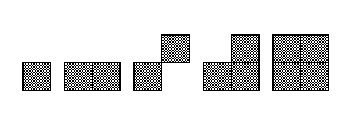
\includegraphics[width=2in]{melaxpieces.jpg}
\caption{Melax's reduced set of pieces}
\label{fig:melaxpiece}
\end{figure}

\begin{figure}[h]
\centering
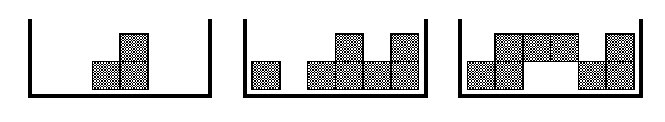
\includegraphics[width=4in]{melaxstates.jpg}
\caption{Melax's reduced environment}
\label{fig:melaxenv}
\end{figure}

Pieces fall from an infinite height. When the working height, which is defined as 2 for this implementation, is exceeded the lowest visible row is dropped and the height incremented by 1. The agent is penalised  -100 for each level it goes above the working height, otherwise it is awarded nothing. Since there was no terminating height, Melax limited his investigations to 10000 pieces per game.

\begin{table}[h]
\centering
\begin{tabular}{|r|r|}
\hline
Game & Height  \\
\hline
    1 &  1485 \\
     2  & 1166 \\
     4  & 1032 \\
     8  &  902 \\
    16  &  837 \\
    32  &  644 \\
    64  &  395 \\
   128  &  303 \\
   256   & 289 \\
\hline
\end{tabular}
\caption{Melax's results for reduced tetris}
\label{mresults}
\end{table}

Table \ref{mresults} shows Melax's results for his implementation of reduced Tetris. As the number of games increased, the agent learnt how to minimise the total height of the pieces in the well and therefore maximised its long term reward.

One possible problem with this implementation, is that by defining rewards for sub-goals such as increasing the working height, we are effectively steering the development of the agent's policy. We have trained the agent to minimise the working height in the well, rather than maximising either the number of completed rows or the number of pieces entering the game. This might actually be the ideal policy for the agent to adopt, especially in the context of our adopted Tetris specifications \citep{tetstand}, but our agent has just lost one potential avenue of exploration.  

Melax's approach was later adopted by \cite{yaeltetris} and extended to include further state space optimisations. These optimisations included regarding only the contours(Figure \ref{fig:contop}), and therefore neglecting all the information beneath the top most row, and the use of symmetry(Figure \ref{fig:symop}) to reduce the state space.  Melax's \citep{melaxtetris} previous results were confirmed, and the further approximations improved the learning results drastically, vindicating their inclusion\citep{yaeltetris}. 

\begin{figure}[h]
\centering
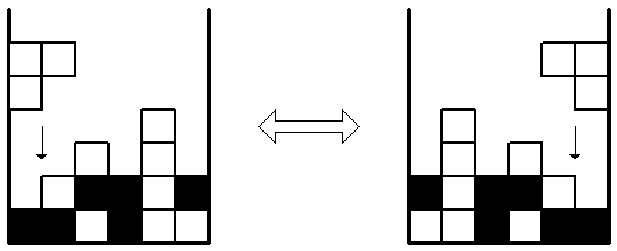
\includegraphics[width=2.8in]{Symetry.jpg}
\caption{\cite{yaeltetris} symmetry optimisation}
\label{fig:symop}
\end{figure}

\begin{figure}[h]
\centering
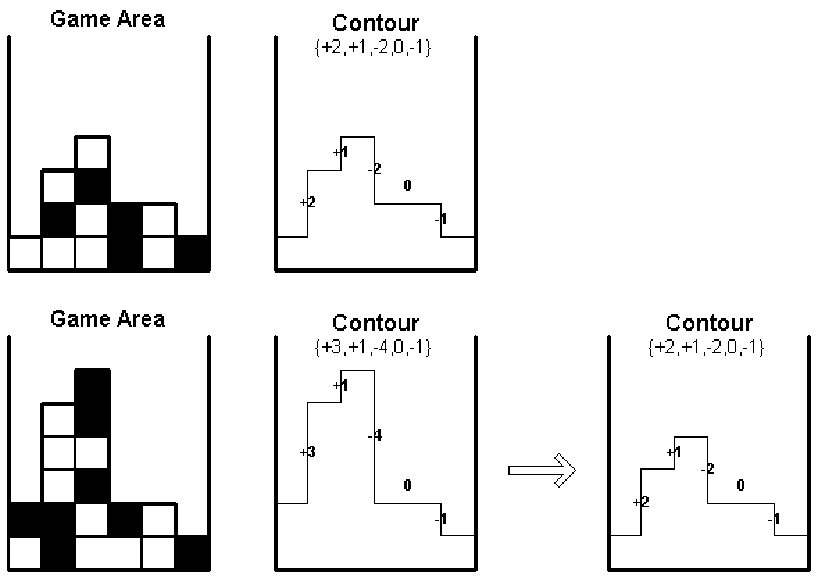
\includegraphics[width=2.8in]{contour.jpg}
\caption{\cite{yaeltetris}contour optimisation}
\label{fig:contop}
\end{figure}

\subsubsection{Full Tetris}
Relational reinforcement learning has been applied to the full Tetris problem by \cite{kurt}. Relational reinforcement learning differs from traditional methods in the structuring of the value function. Rather then storing every possible state in a table, the relationship between the elements in the environment is utilised in developing a reduced state space. This state information is then stored in a decision tree structure.   He approached the problem with three separate relational regression methods \citep{kurt} he had developed over the course of his thesis. The first of these regression methods had already proven itself in the course of the thesis with the successful extension of reinforcement learning to Digger\footnote{Another game with a large state space}. 
 
\cite{kurt} did not use a straight-forward attribute vector to represent the Tetris state space\footnote{This information regarding state representation was kindly supplied by the author via email, and is taken directly from the correspondence}.

He used the following features in developing his decision tree based learner : \\

\begin{itemize}
\item{ blockwidth, blockheight which specify the width and height of the
falling block respectively.}
\item{ topBlock which returns the height of the wall at a given column.}
\item{ holeCovered: whether there is a hole in the wall at a given column.}
\item{ holeDepth which returns the depth of the topmost hole in the wall at a
given column.}
\item{ fits: whether the falling block fits at a given location with a given
orientation.}
\item{ increasesHeight: whether dropping the falling block at a given
location with a given orientation increases the overall height of the wall.}
\item{ fillsRow and fillsDouble: whether the falling block completes a line
(or two lines) at a given location with a given orientation.}
\end{itemize}
He used the following features in developing his instance based learner : \\
\begin{itemize}
\item{ The height of individual columns.}
\item{ The maximum, average and minimum height of the wall and the
differences between the extremes and the average.}
\item{ The height differences between adjacent columns.}
\item{ The number of holes and canyons of width 1.}
\item{ The average depth of holes.}
\end{itemize}

\begin{table}[h]
\centering
\begin{tabular}{|r|r|r|}
\hline
Regression method & Learning games & Completed rows  \\
\hline
RRL-TG	&	5000	& 	10   \\
\hline
RRL-RIB  &  50  & 12  \\
\hline
RRL-KBR  &  10-20  & 30-40  \\
\hline
\end{tabular}
\caption{Relational regression results \citep{kurt}}
\label{abc}
\end{table}

The RRL-RIB reached its optimal policy within 50 training games. In 450 subsequent training games this policy was not improved upon. RRL-KBR reached a better policy, earlier then the other regression methods. It then rather unexpectedly unlearnt its policy after a further 20-30 learning games.

Since this is actually a full implementation of Tetris it can be compared against other AI results, where the best (comparable) methods score in the region of 650 000 completed rows\citep{tetstand}. These results are not impressive in the light of the competition, and very poor even by human standards. Driessens attributes the poor functionality to Q-learning, stipulating that Q-learning requires a good estimate of the future rewards in order to function properly and that the stochastic nature of Tetris severely limits the accuracy of these estimates. Since his regressions methods were derived from Q-learning, this inadequacy impacted on all of his methods. Q-learning in known to be unstable\citep[pg. 4]{keepaway,thrun93issues} when incorporated in function approximation, and this could certainly have contributed to the poor performance witnessed in the above results.

\subsubsection{Work in progress}

There is ongoing research into possible methods of solving Tetris using reinforcement learning. An approach known as CB-Mineral that is similar to that used by Tesauro \citep{tdgammon} is being generalised and has Tetris as its first line of application\citep{cuttingtet}. This involves utilising reinforcement learning in training the weights of a neural network, rather then engaging in supervised learning, and effectively uses neural networks as a form of function approximation.

\section{Possible implementation}

The first step will be to try repeat the achievements of \cite{melaxtetris} and \cite{yaeltetris}. If learning is achieved, then extending the agent will require a complete redefinition of the environment and the value function, but will show the successful implementation of basic reinforcement learning.

The Tetris well is 20 blocks high and 10 blocks wide, and therefore has 200 blocks that can either be empty or occupied, resulting in $2^{200}$ possible states. This number is huge and any linear value function spanning the complete state space of Tetris is computationally infeasible\citep{tetrisconstraint}.

Before considering a reduction in the state space of the game we ought to clarify that the original state space is capable of storing all the information required to successfully solve the problem.  

There is an ideal action in every state, depending on the current state and the current tetromino. Since the next tetromino is stochastically selected after the state transition, the next state is not considered in the context of the next tetromino. Implementing Tetris with one piece look ahead would lead to an array of $2^{200}$ states for each tetromino, but would guarantee the possibility of the agent following optimal policy. Without the one piece look ahead, the agent may well select a state with a high value and then be dealt a tetromino that is useless in the current state. The implication of this is that the agent will always be at the mercy of the stochastic process selecting tetrominoes, and may well change its policy off the optimal policy as a result of this. With no look ahead, only one value need be associated with each state and  an array of $2^{200}$ values contains all the information required to achieve an optimal policy.

This representation contains a large amount of redundant information, and it is a non-trivial task to reduce the state space without impairing the performance of the agent or losing pertinent information. 

The same configuration of tetrominoes can be shifted up or down in the well, and would require the same tetromino placement in each case. This lack of generality leads to slower learning, as the same tactics have to be learnt at different heights and this also increases the state space drastically. As a human, one does not look at the exact height at which a pattern occurs. An example of a simple reduction would be to reduce the height of the well into coarser discrete areas. This would enable the agent to factor height into its considerations, without drastically increasing the state space of the game.

Calculating the possible transition states is made fairly straightforward by considering afterstates\citep{kurt}. This involves varying the tetromino through its complete range of orientations and translations, and dropping each variation in the well. This will return a value for every possible translation/rotation combination and the policy can select within these values with ease.

The most intuitive policy to use would be the softmax policy since there will be a large state space to explore, regardless of state space reduction. Using an $\epsilon$-greedy method would effectively blindfold the agent in its selection of exploratory routes, and lead to a great deal of wasted exploration. The more attractive a state appears to be, the more it will be explored.

Over-extending the reward function can prejudice the development of the value function, and therefore the policy of the agent. Placing pieces over openings is an obvious candidate for punishment, as it could be argued that this could never be utilised to advance the abilities of the player. Punishing the player for increasing the working height would result in an agent that completes rows, but would steer the agent away from effective stacking in circumstances where repeated Z or S pieces are received. Rewarding an agent for completing rows leaves the agent's activities up to itself, although states that lead to completion will be selected more often, and explored more thoroughly.

\section{Conclusion}

Reinforcement learning has been successfully applied to many problems, and is broad enough in its scope that historical failures to successfully apply it to a problem could be due to implementation faults. Previous failed attempts have indicated the complexities associated with tackling Tetris, but have not revealed the whole field of reinforcement learning to be unsuitable or ill qualified to learn Tetris. Tetris is an interesting game that has inspired a lot of academic research, and could benefit from the existence of an uninhibited potentially non-conventional player. 

\bibliography{litreview}
\end{document}

